%%%%%%%%%%%%%%%%%%%%%%%%%%%%%%%%%%%%%%%%%%%%%%%%%%%%%%%%%%%%%%%%%%%%%%%%%%%%%%%%
% uncertainties.tex: Chapter on uncertainty:
%%%%%%%%%%%%%%%%%%%%%%%%%%%%%%%%%%%%%%%%%%%%%%%%%%%%%%%%%%%%%%%%%%%%%%%%%%%%%%%%

\chapter{\texorpdfstring{\phistar}{Phistar} Uncertainties}
\label{Uncertainties_chapter}

\begin{figure}[!htbp]
    \centering
    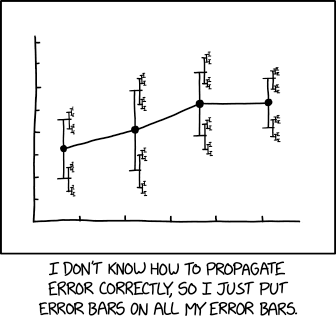
\includegraphics[width=.6\textwidth]{figures/uncertainties/uncertainty.png}
    \caption[]{The propagation of uncertainty can be complicated, as this  {\tt xkcd}\cite{xkcdComic} alludes, }
    \label{fig:xkcd4}
\end{figure}{}
The uncertainty of a measurement is as important as the measurement itself. Without knowing the uncertainty, it is not possible to quantify the theory's agreement with data. This chapter describes how these uncertainties are included in both data and simulation.

\section{Propagation of Statistical Uncertainty}
The statistical uncertainty of a measured number of events, $N_{i}$, is trivially defined by $\sqrt{N_{i}}$. However, the measured \phistar distribution is not directly comparable to simulation. Rather, the measured \phistar distribution is unfolded first, which leads to the need to propagate the statistical uncertainty into the unfolded results. This calculation is performed by RooUnfold which propagates the statistical uncertainty of the data through the unfolding matrix and outputs a covariance matrix. Due to the small amount of bin migration it was decided to just use the diagonal of the covariance matrix as the unfolded statistical uncertainty. Two tests were preformed to validate this assumption. 
\subsection{Validation of the Statistical Approach}
A test was  preformed to prove the triviality of the off diagonal terms of the statistical covariance matrix. This test used simple ``toy" Monte Carlo samples that were created using a central \MADGRAPH \phistar distribution to create new Monte Carlo distributions. Each new toy Monte Carlo distribution was generated by taking each bin of the original \MADGRAPH distribution and varying it randomly using a Gaussian distribution, centered at the bin's original value, and using the bin's uncertainty as the width of the Gaussian distribution. This method was used to create 500 new distributions with each distribution unfolded using the \POWHEG distribution. The resulting bin values along with their deviation is compared to the central result whose deviation comes directly from the diagonal of the covariance matrix for the statistical data.  With the results shown in Fig \ref{fig:BinMigrationWToys}, the correlation between bins due to statistical fluctuations in the unfolded sample have minor effects on the uncertainty of each bin. 

\begin{figure}[!htbp]
    \centering
    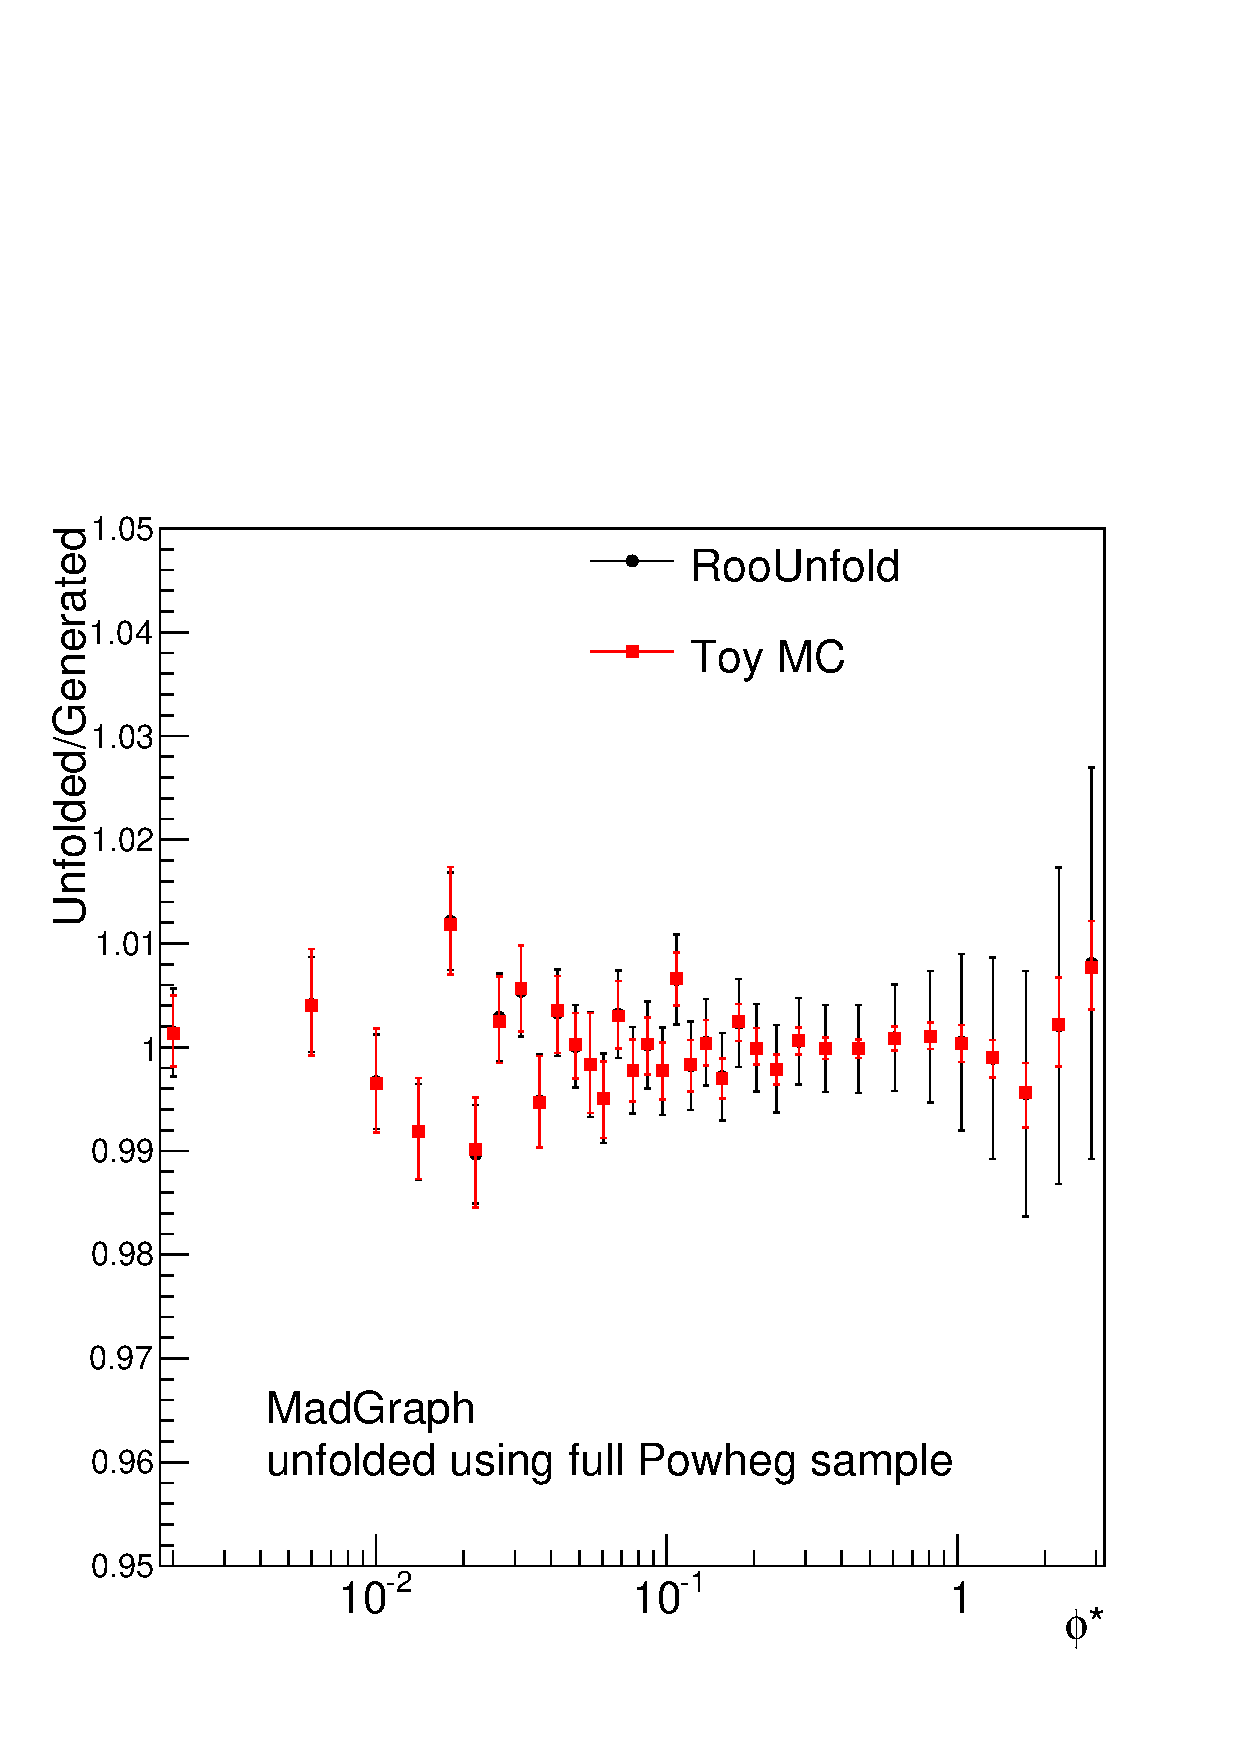
\includegraphics[width=.8\textwidth]{figures/Unfolding/BinM_PM_ALL.pdf}
    \caption[
        BinMigration
    ]{
A MadGraph sample unfolded using \POWHEG. The black shows the results from RooUnfold with the uncertainty taken from the Diagonal of the covariance matrix that RooUnfold produces. The red is the average position of the result from unfolding using the Toy samples, where the red line defines one standard deviation, defined as the spread of the central 68.2\% of the values in that bin. 
    }
    \label{fig:BinMigrationWToys}
\end{figure}
\subsection{Cross Check of Simulation Statistics}
This test was done to prove that the output statistical uncertainty of RooUnfold does not include and is not affected by the statistics of the simulation used to unfold the sample.  This was done twice, once with 5000 randomly chosen \POWHEG events, and a second time with 50000 randomly chosen events. As was done with the first test, 500 toy samples were created and unfolded using these two subsamples, with the results shown in Fig \ref{fig:BinMigrationWToysSmallerSamples}. By observing both figures it can be seen that there is a larger fluctuation in the data when a smaller Monte Carlo sample is used to unfold the data, however the error bars on the unfolded data are still on the order of 1\% because they only include the propagated uncertainty of the unfolded results. The red error bars, however, show the standard deviation of the unfolded toy Monte Carlo samples, which is sensitive to the lack of statistics in the sample used for the unfolding. 

\begin{figure}[!htbp]
    \centering
   \begin{subfigure}[b]{0.49\textwidth}
     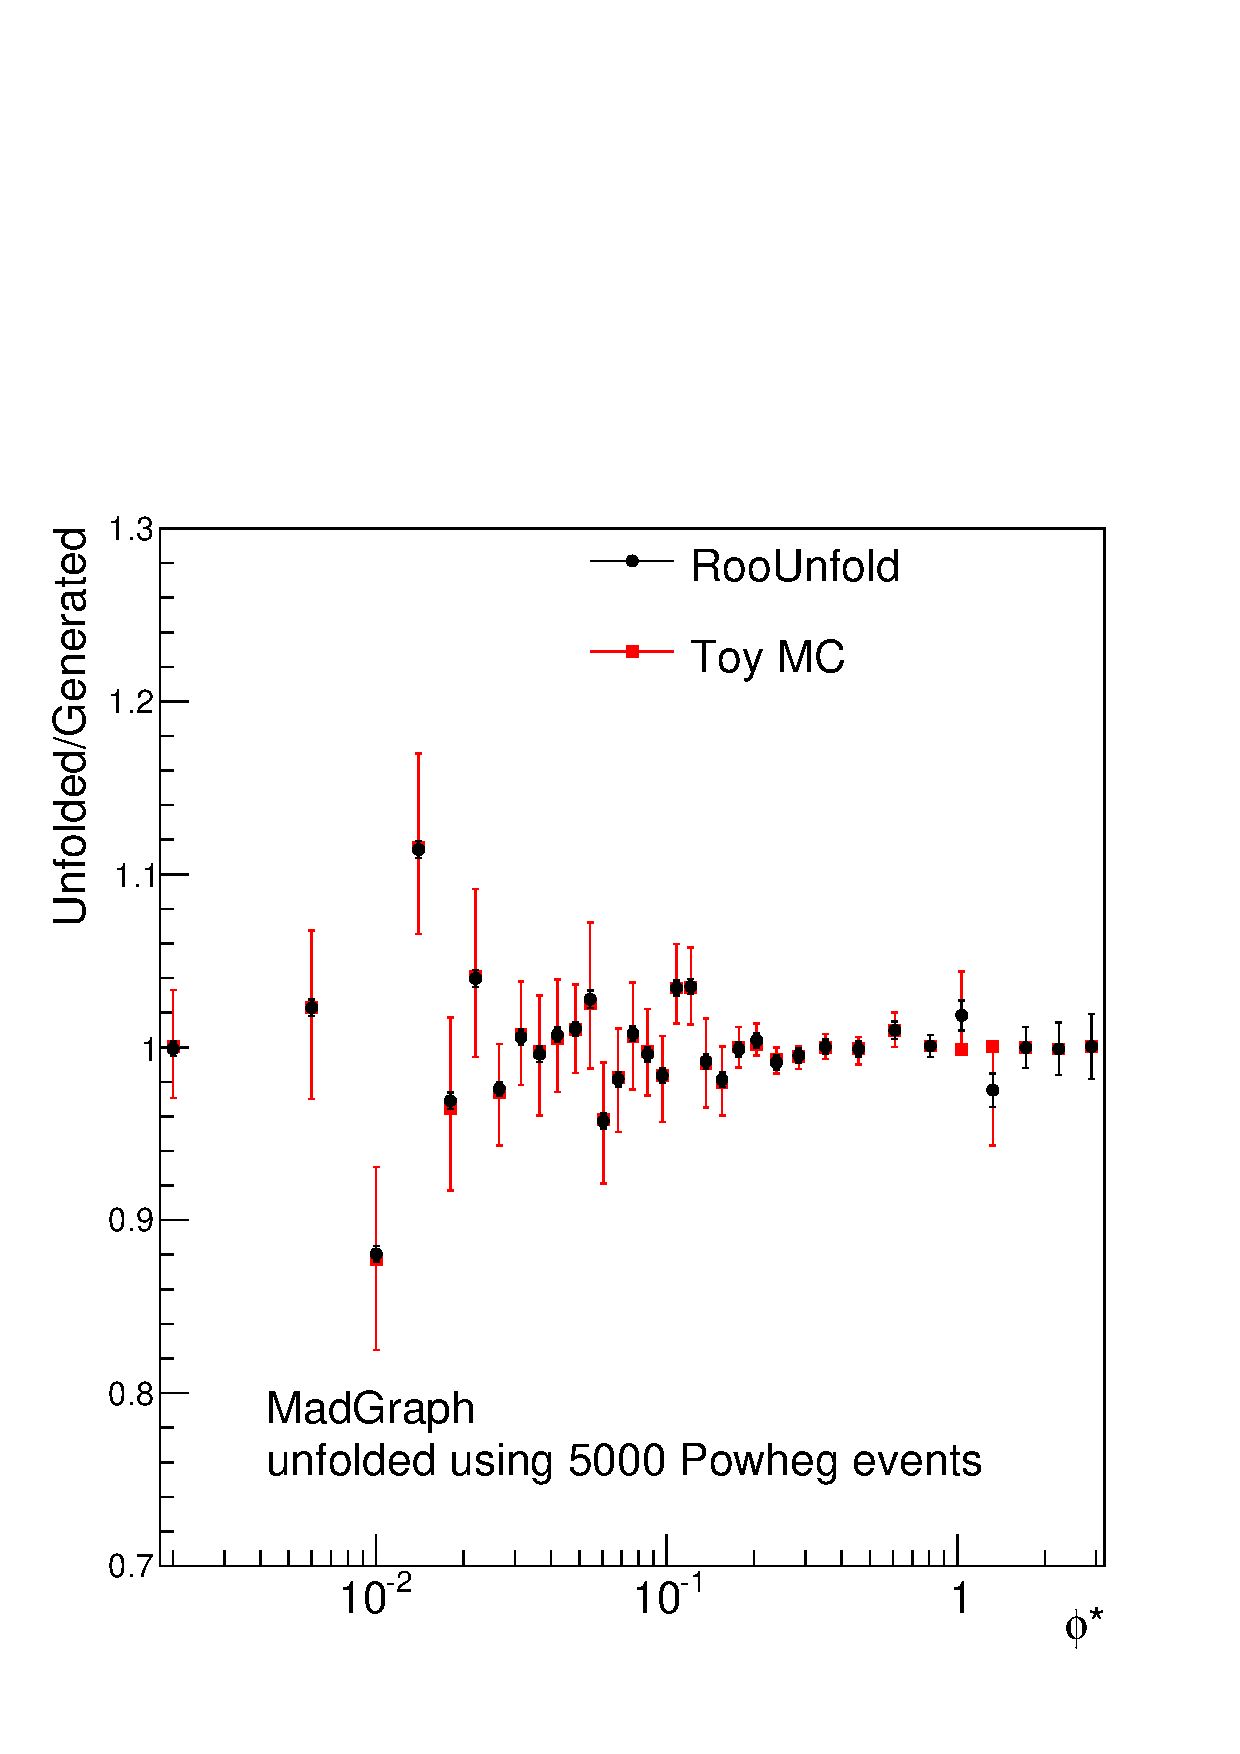
\includegraphics[width=\linewidth]{figures/Unfolding/BinM_PM_5000.pdf}
     \caption{}
    \end{subfigure}
    \begin{subfigure}[b]{0.49\textwidth}
     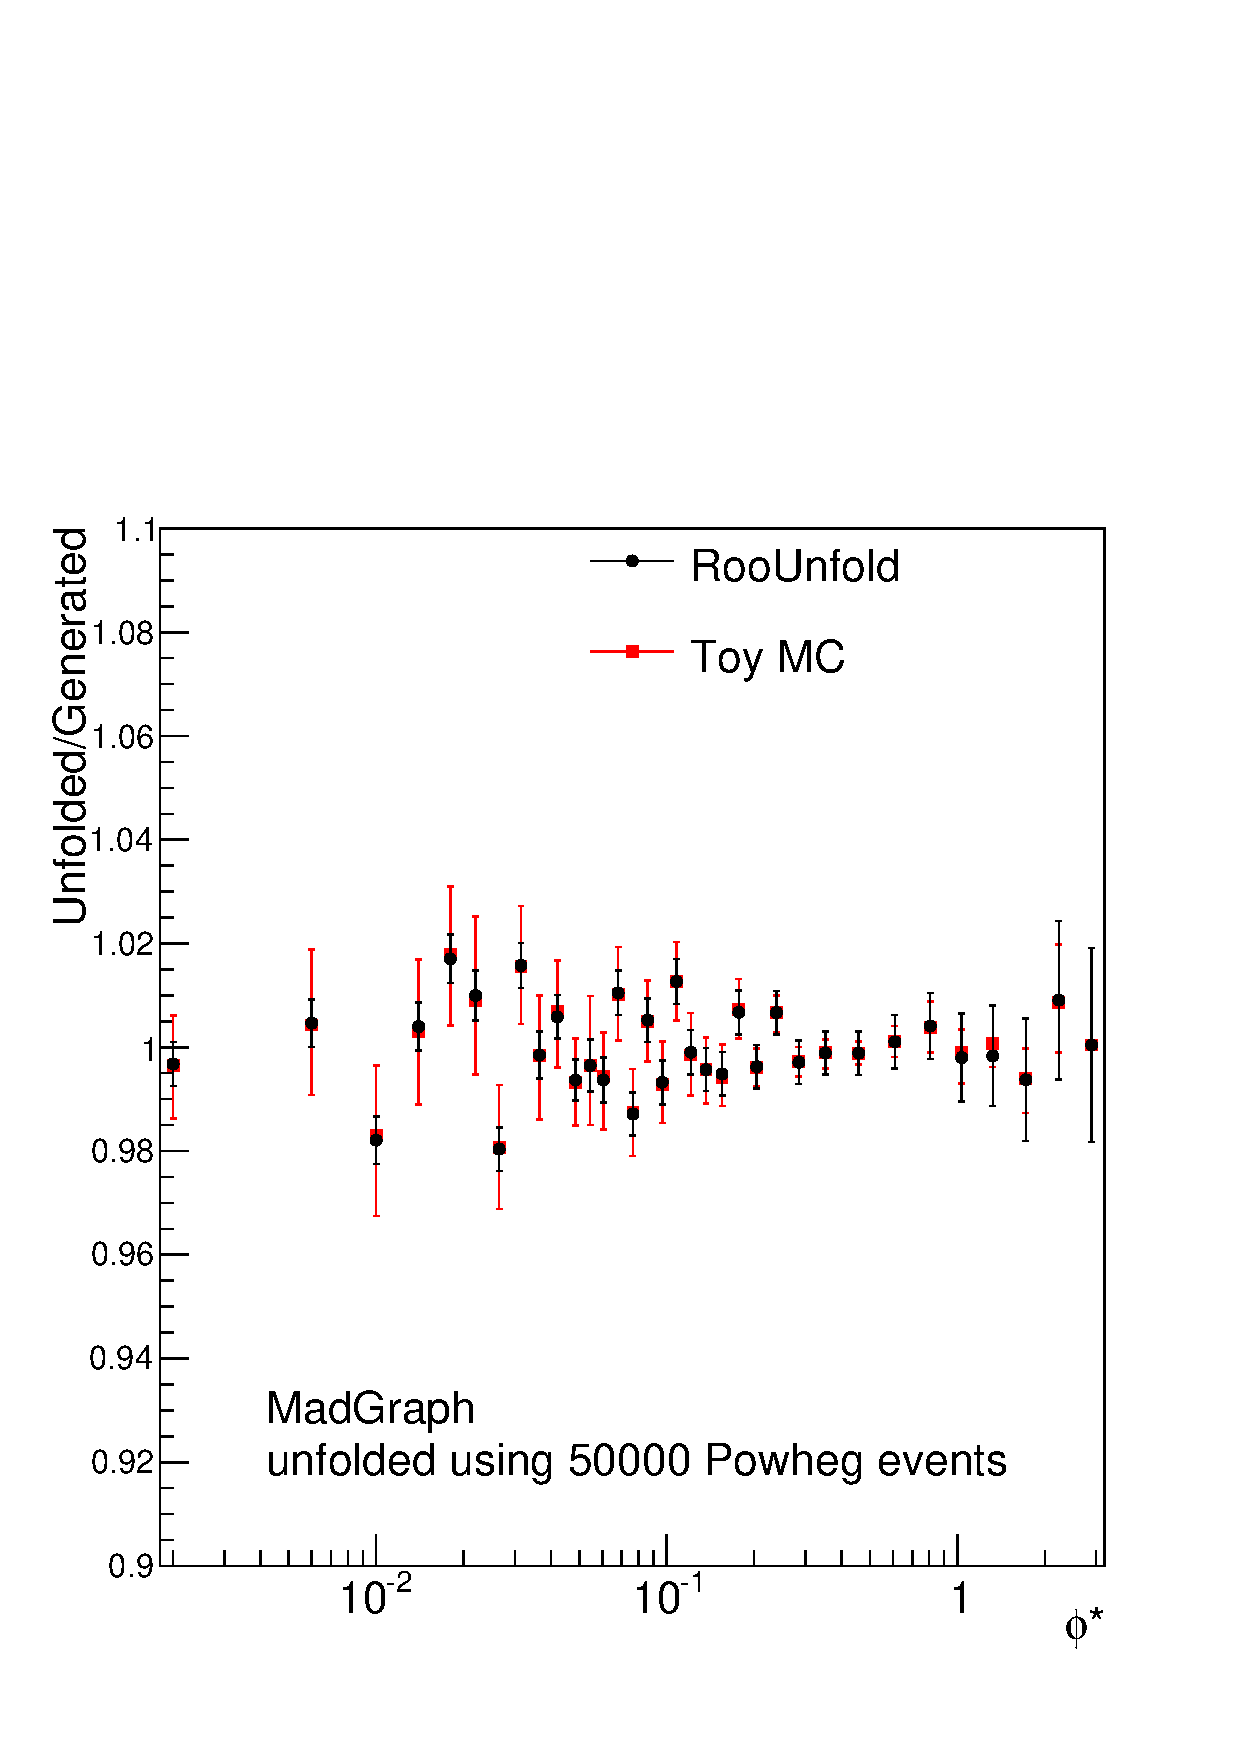
\includegraphics[width=\linewidth]{figures/Unfolding/BinM_PM_50000.pdf}
     \caption{}
    \end{subfigure}
    \caption{500 samples created using a central \MADGRAPH where each bin was fluctuated independently based on its statistical uncertainty. These samples were unfolded using two \POWHEG subsamples, with the left plot unfolded using a \POWHEG sample with 5000 events and the right with a sample containing 50000 events. The black points are the central Monte Carlo sample and the black bars show the propagated uncertainty using RooUnfold, while the red points are the average value of the toys and the red error bars are the standard deviation of the unfolded toys.}
    \label{fig:BinMigrationWToysSmallerSamples}
\end{figure}




\subsection{Normalized Statistical Uncertainty}
Statistical uncertainty decreases in the normalized data distributions. The uncertainty of the ith bin in a normalized distribution is calculated using the equation:

\begin{equation}
(\epsilon_i^{norm})^2
=
(\epsilon_i^{abs}\times(\frac{1}{\sigma}-\frac{\sigma_i}{\sigma^2}))^2+\sum\limits_{i\neq j}(\epsilon_j^{abs}\times \frac{\sigma_i}{\sigma^2})^2;
\end{equation}
$\epsilon^{abs}_j$ is the statistical uncertainty of bin $j$ for the absolute distribution, $\sigma_{i}$ is a particular bin's cross-section, and $\sigma$ is the overall cross-section given by the integral of the distribution. 

\section{Unfolding and Monte Carlo Statistical Uncertainty}
Although a \Z simulation sample was used to unfold the data, according to Ref \cite{dagostini_1995} it is not necessary for the distribution that is used to unfold the data to be correct. Only the relationship between generated and reconstructed bins is required to be accurate. This was tested by placing events of a \POWHEG sample into a histogram of bin width $\Delta\phistar=0.001$. The weight for each of these bins was set to be inversely proportional to the number of events in the bin, creating a flattened distribution. This new flattened distribution was used to unfold the \MADGRAPH sample. As can be seen in Fig. \ref{fig:BinMigrationWFlatPowheg}, there is no significant deviation. Therefore our, uncertainty due to unfolding is calculated only using the uncertainty due to simulation statistics. 
\begin{figure}[!htbp]
    \centering
   \begin{subfigure}[b]{0.49\textwidth}
     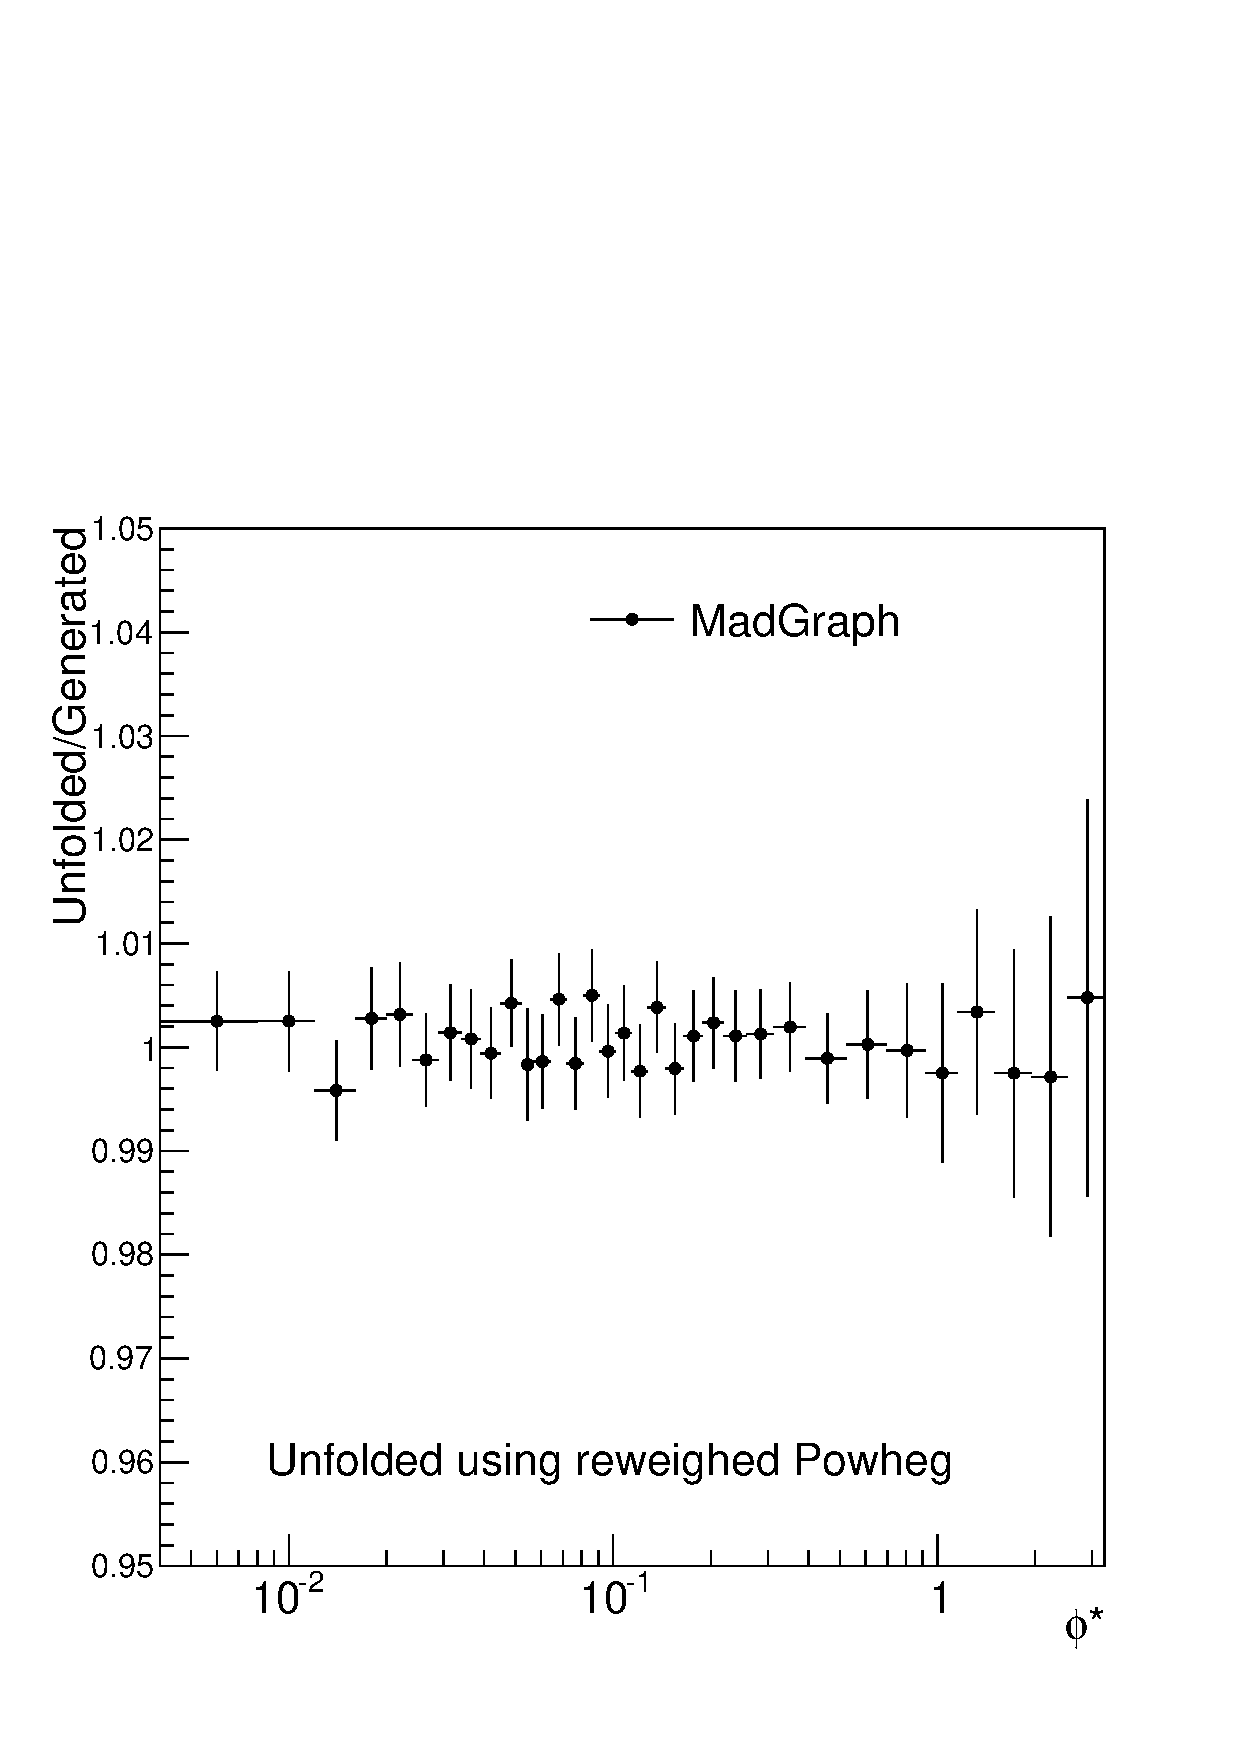
\includegraphics[width=\linewidth]{figures/AnalysisSection/MadUnfolFlatPH.pdf}
     \caption{}
    \end{subfigure}
    \begin{subfigure}[b]{0.49\textwidth}
     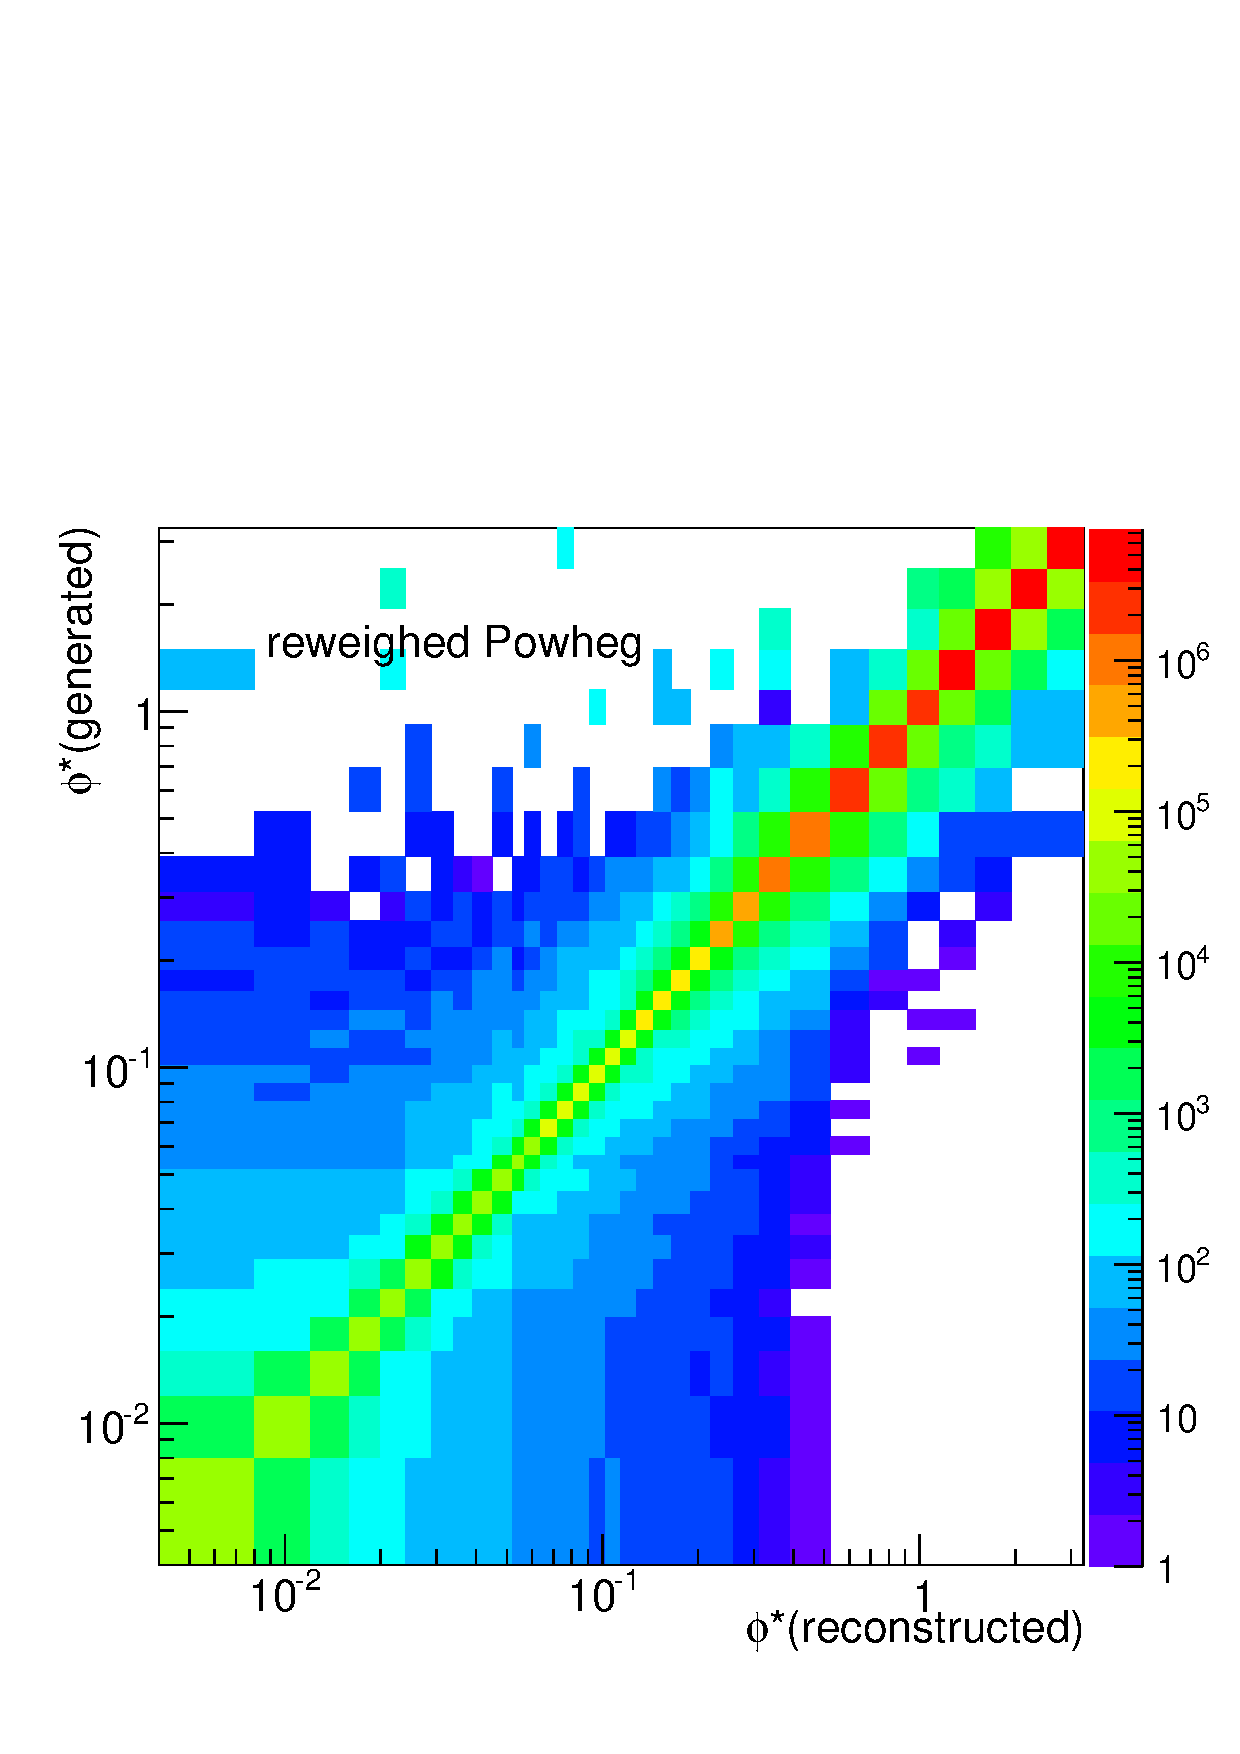
\includegraphics[width=\linewidth]{figures/AnalysisSection/UnfoldWithFlatMatrix.pdf}
     \caption{}
    \end{subfigure}
    \caption{Left: A ratio of unfolded reconstructed \phistar distribution of a \MADGRAPH \Ztoee sample over the generated distribution for the same sample. The sample was unfolded with a flattened \Ztoee \POWHEG sample.  Right: The bin migration matrix produced using the flattened \POWHEG distribution.}
    \label{fig:BinMigrationWFlatPowheg}
\end{figure}

The uncertainty due to the statistics of the simulation sample used to create the unfolding matrix is not included by RooUnfold's covariance matrix. In order to calculate the uncertainty of the unfolded data due to the statistical uncertainty of the sample used to unfold the data, a method similar to the one used for checking the propagation of statistical uncertainty was used. Five hundred Monte Carlo samples were created using the same method as above, and used to unfold the data. An example is shown in Fig. \ref{fig:UnfoldMonte CarloStatErrorExample}. The standard deviation of this plot is used as the unfolding uncertainty, and is around 0.5\% for the majority of the bins, though at high \phistar values it increases to around 1\%. 

\begin{figure}
    \centering
    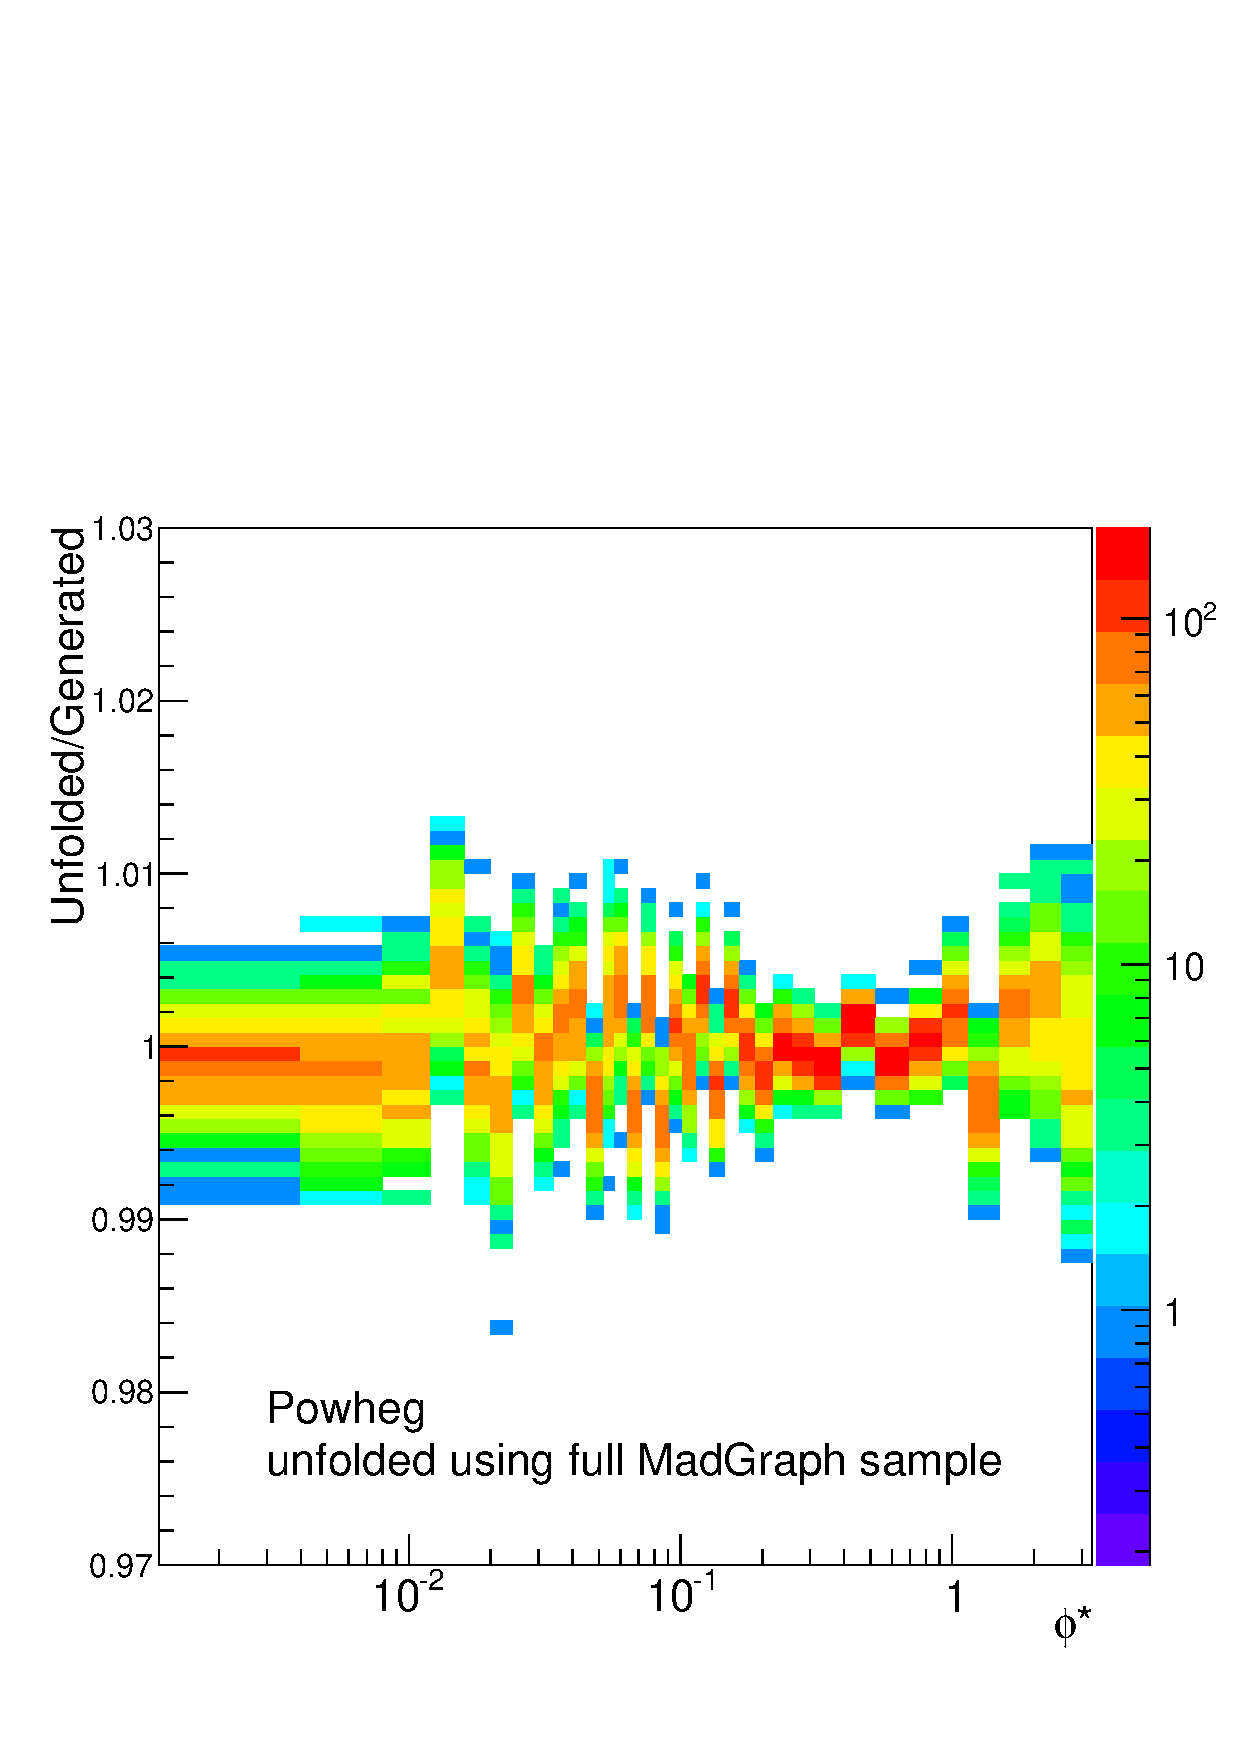
\includegraphics[width=\textwidth]{figures/Unfolding/BM_2D_PM_FULL.pdf}
    \caption{An example showing the unfolding results of a \POWHEG sample after being unfolded by 500 \MADGRAPH samples.}
    \label{fig:UnfoldMonte CarloStatErrorExample}
\end{figure}



\section{Additional Uncertainties}
In addition to statistical uncertainties, there are also systematic uncertainties. These uncertainties, such as those from theory, include the cross-section of backgrounds, as well as rates of FSR. Another source of uncertainty comes from the detector. This includes luminosity, as well as the reconstruction and measurement of the electron, such as its momentum and its direction.
\subsection{Luminosity}
All measurements of the absolute rates, or the cross-section, must be normalized to the exposure of the detector which is called the integrated luminosity of the data sample. 
In order to measure the integrated luminosity, CMS uses the number of charged particles produced in all interactions. The majority of interactions do not produce anything of interest; the ever-present QCD interactions create a spray of charged particles. The luminosity is calculated by measuring the occupancy of the pixel tracker \cite{cms_lumi_2013}\cite{vandermeer_1968}. 
The integrated luminosity of the data sample of CMS has a 2.6\% uncertainty. This uncertainty dominates the absolute \phistar distribution, being larger then  all other uncertainties by more than a factor of two, except in the last few bins. Fortunately this uncertainty is fully correlated between all \phistar bins, so  normalizing cancels out the  the uncertainty, and is only involved slightly in the background subtraction. Due to the small backgrounds and large uncertainties in the cross sections used in the background subtraction, the luminosity uncertainty has trivial effect on the normalized distribution.



\subsection{Trigger, Reconstruction, and  Identification Scale Factors}
As mentioned in Sec \ref{sec:Measuing_Efficiency}, scale factors are used to compensate for differences between the simulated detector and the real one. The uncertainty is calculated by creating 500 toy Monte Carlo samples for each type of scale factor. For each toy, a new scale factor is chosen from a Gaussian centered at the nominal scale factor with the width being the uncertainty of the scale factor. The uncertainty is taken from the central 68.2\% of results from the toys. This is done independently for all scale types of scale factors, and then the final uncertainties are added in quadrature. 



\iffalse 
\section{PDF and Cross Section Uncertainty}
As mentioned in sec \ref{sec:pdf}, quarks do not have a set momentum fraction inside the proton. Because the amount of momentum that these quarks have effects on the \Z bosons momentum, \phistar is dependent on the PDFs that are used to generate the Monte Carlo samples.

For \POWHEG The uncertainty due to the PDF is calculated using the recommendation of the \Software{PDF4LHC} working group  \cite{Botje:2011sn}. In order to calculate this uncertainty each event was given new 26 weights, creating 26 \phistar distributions. These weights were created using the \PDFWeightProducer on the  \POWHEG sample using the \Software{CT10} \Software{PDF}. These weights were produced by the \Software{CT10} collaboration for the purpose of calculating the PDF uncertainty. These are done to test 13 different variables used by the software, with one weight adjusting the variable up and a different weight decreasing the value. The difference between the nominal distribution and the new distribution is taken as the uncertainty. The uncertainties are put into two groups by whether the weight is related to a variable that had increased verse a variable that had been decreased. Each group then adds all its members uncertainties in quadrature. For each bin the uncertainty is taken as the value of the largest group.
\fi


\subsection{Background Uncertainty}
The background uncertainties are estimated by varying the theoretical cross sections of the different backgrounds. Due to the very small size of the backgrounds for this study, it was decided to overestimate their uncertainty to remove doubt of their unimportance. The uncertainty due to \ttbar is calculated by varying the theoretical cross section by 10\%. The WZ and ZZ cross-sections are varied by 20\% and the QCD and W+jets are varied by 100\%. The new distributions are used in the background subtraction to create two new data distributions that are then unfolded. The uncertainty is defined as the difference between this new unfolded result and the original. The resulting uncertainties are added in quadrature. All other uncertainties due to background are negligible. 
\subsection{Pileup Uncertainty}
As discussed in Sec \ref{Sec:SimRecon}  additional soft pp interactions are added to events in order to simulate the normal bunch crossing where multiple protons interact. These events are then reweighted so that this can match the actual experimental data. The uncertainty due to this re-weighting is calculated by varying the inelastic proton-proton cross-section up and down by 5\%. The full unfolding process is then performed using these two new samples, with the pileup uncertainty defined as the largest difference between the new unfolded distributions compared to the original.
\subsection{Lepton \texorpdfstring{\pt}{PT} Scale Uncertainty}
The variable \phistar was chosen due to it not being dependent on the \pt measurement of either lepton. Despite this, mismeasurements of the \pt can effect the overall distribution of \phistar. This is due to the acceptance requirements, since it includes \pt requirements. To study the effect of this, we vary the \pt of all electrons up and down by 0.3\%, which is a conservative estimate of the uncertainty of \pt scale. The largest difference for each bin between these new distributions and the nominal distribution is taken as the uncertainty. This leads to a \pt scale uncertainty between $0.07\%$ to $0.17\%$ for the absolute cross section, while the corresponding uncertainty on the normalized cross section is less than $0.1\%$ for all bins.
\subsection{Final State Radiation Uncertainty}
As mentioned in Section \ref{sec:StateRad} FSR occurs when one of the leptons emits a photon. Although unfolding the distribution accounts for this, the unfolding matrix is dependent on the simulation model. Therefore, uncertainties in how well the simulation  models FSR must be propagated. The uncertainties are calculated using \FSRWeightProducer which weights events in an attempt to compensate for missing QED calculations in \PYTHIA.  A new \phistar distribution is created using these weighted events and then compared to the original distribution. The difference between the distributions is taken as the FSR uncertainty. The FSR uncertainty was found to be $<0.013\%$ for the absolute distribution and $<0.011\%$ for the normalized distribution.


\section{Uncertainty Plots}
Each of the uncertainties described is combined in quadrature to show the total uncertainty. Plots showing the scales of uncertainties are shown in Fig \ref{fig:uncertainty}. As can be seen from these plots for the absolute case, the luminosity uncertainty dominates, with all other uncertainties having an effect on the absolute total uncertainty of less than 20\% . For the normalized case, the uncertainty is mostly dominated by statistics, either directly, or in the case of unfolding indirectly, though in higher \phistar other uncertainties start to rise. 

\begin{figure}
    \centering
    \begin{subfigure}[b]{0.49\textwidth}
     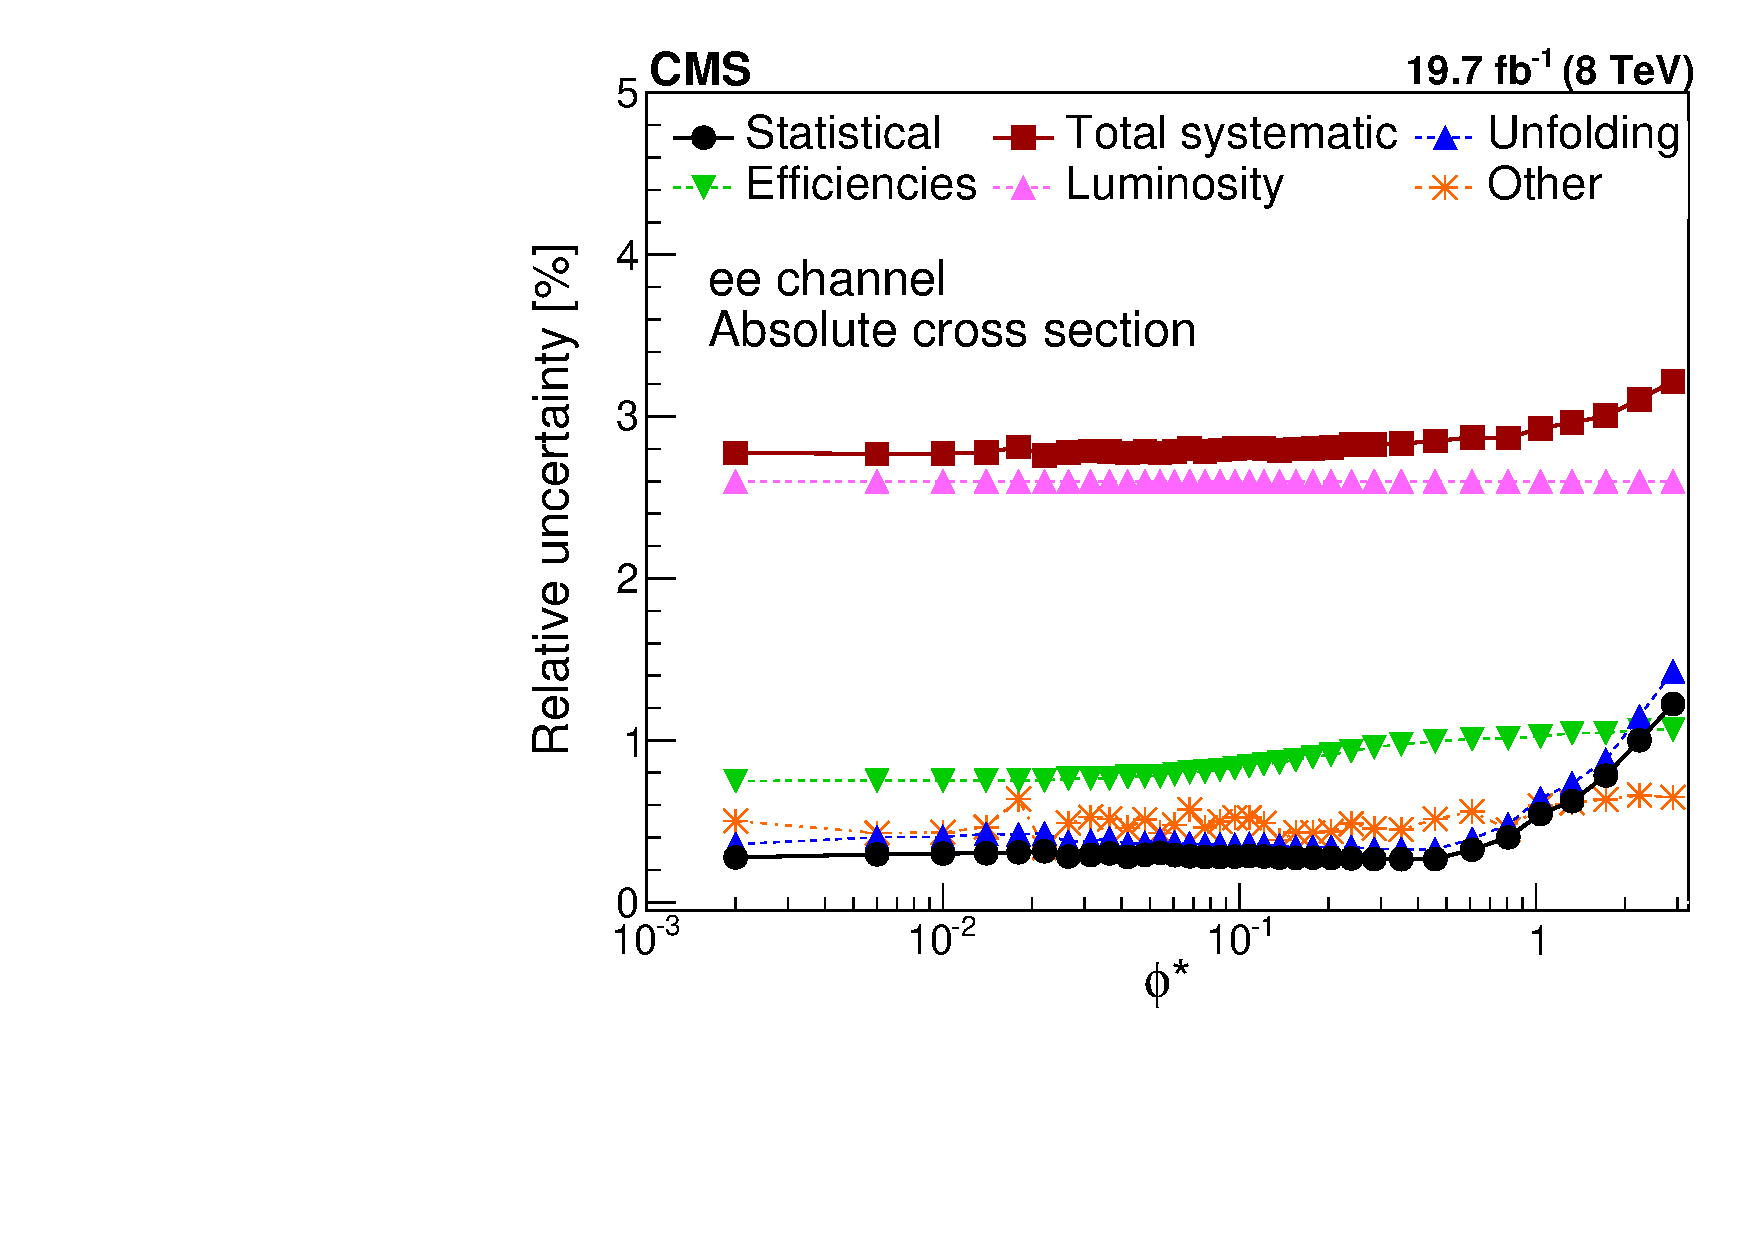
\includegraphics[width=\linewidth]{figures/uncertainties/UncertaintyElecAbs.pdf}
     \caption{}
    \end{subfigure}
    \begin{subfigure}[b]{0.49\textwidth}
     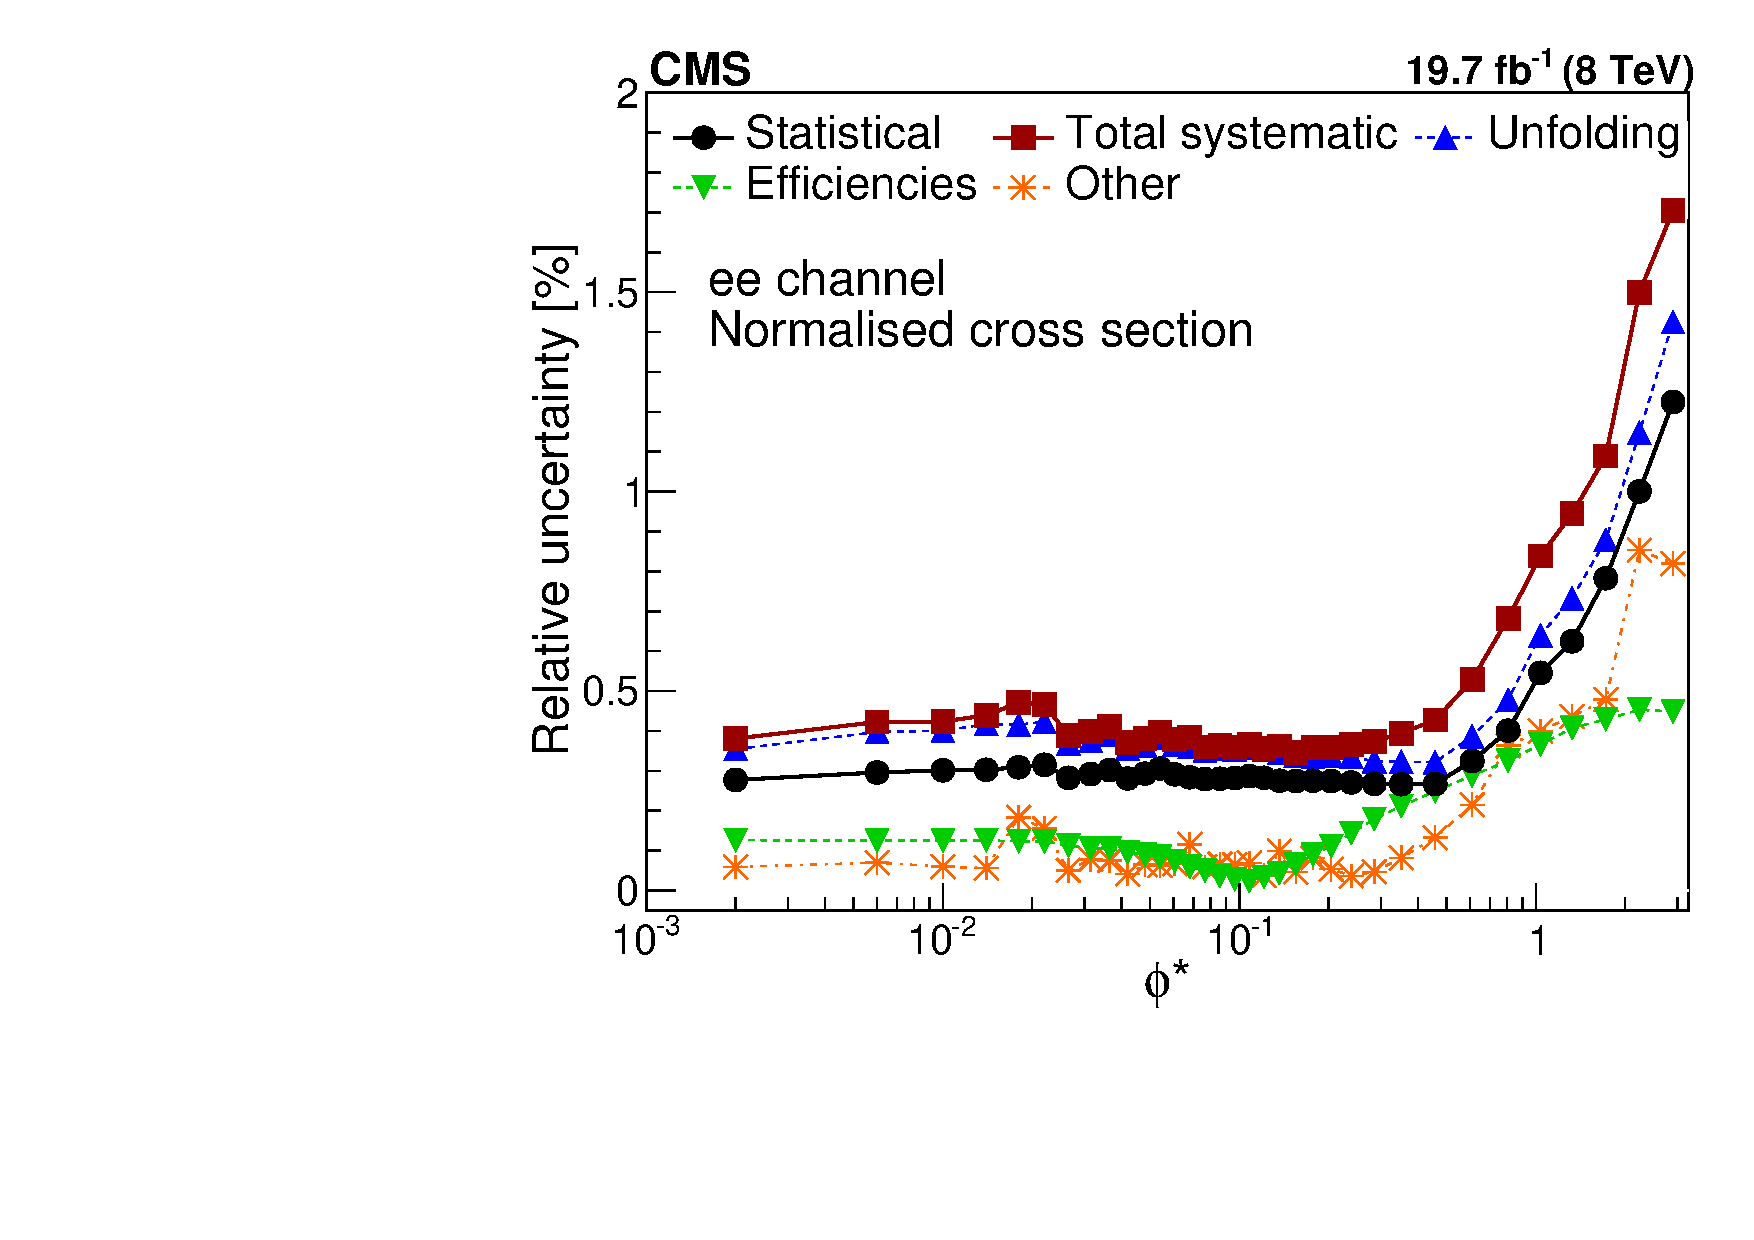
\includegraphics[width=\linewidth]{figures/uncertainties/UncertaintyElecNorm.pdf}
     \caption{}
    \end{subfigure}
    \begin{subfigure}[b]{0.49\textwidth}
     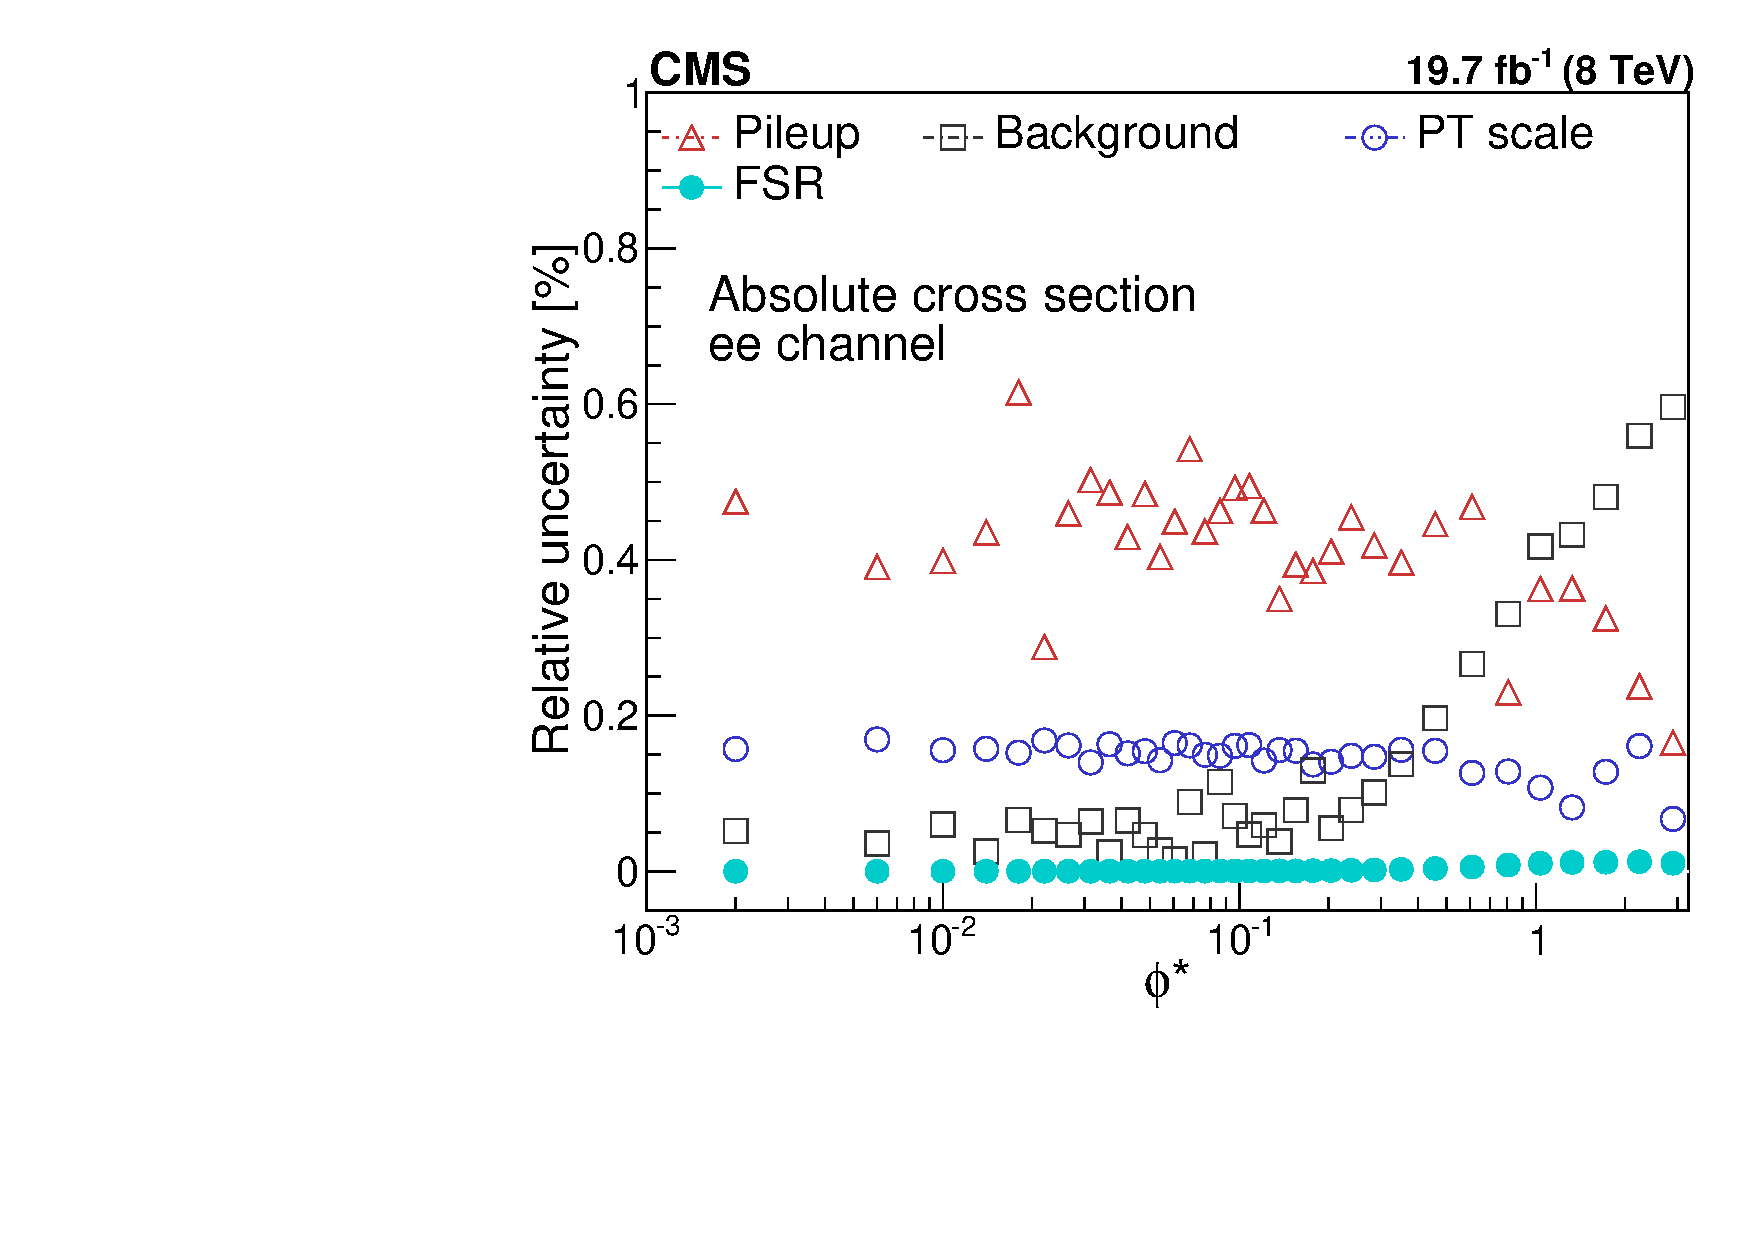
\includegraphics[width=\linewidth]{figures/uncertainties/UncertaintyElecAbsType0.pdf}
     \caption{}
    \end{subfigure}
    \begin{subfigure}[b]{0.49\textwidth}
     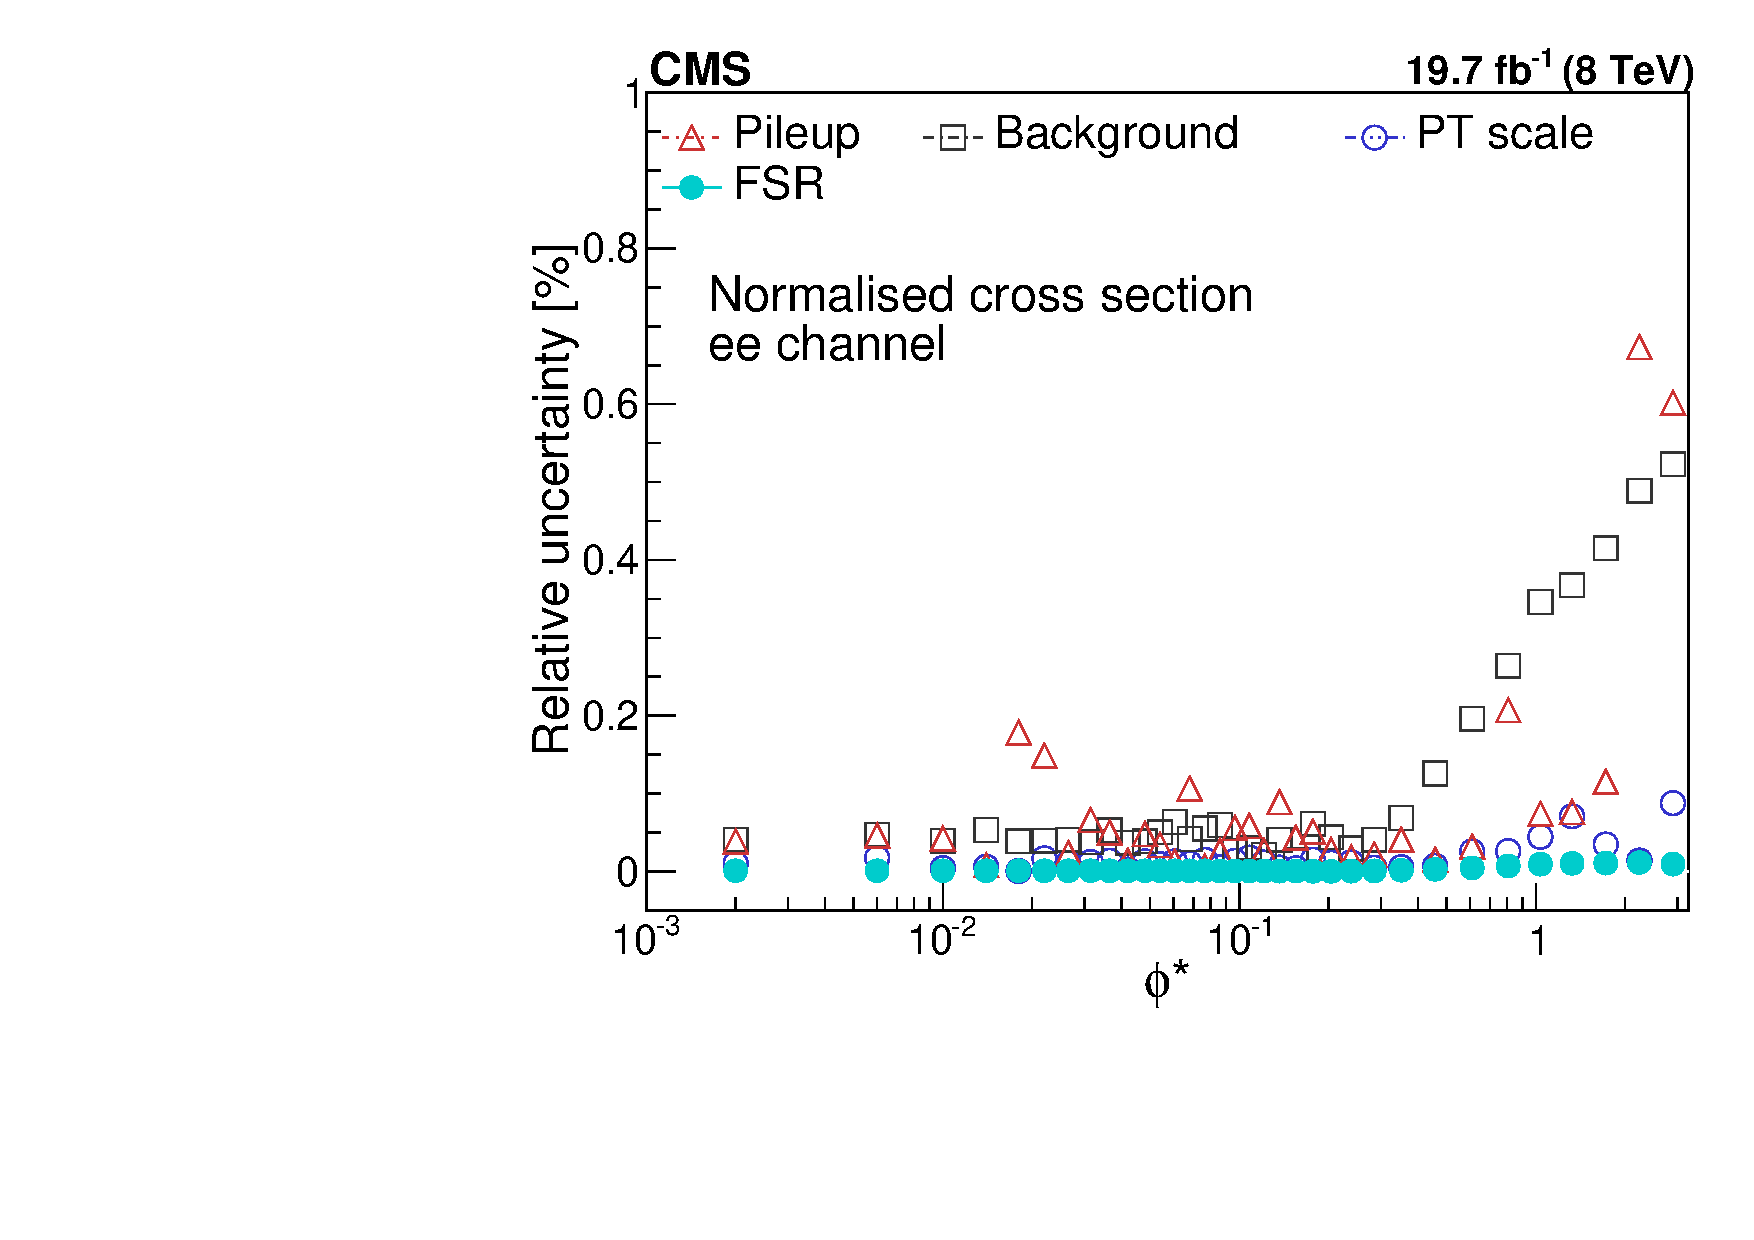
\includegraphics[width=\linewidth]{figures/uncertainties/UncertaintyElecNormType0.pdf}
     \caption{}
    \end{subfigure}
    \caption{The top figures show the variation of the statistical and systematic uncertainties with \phistar. The uncertainties from background, pileup, electron energy scale, and from QED-FSR modeling are combined under the label ``Other".  The bottom plot shows each of these ``Other" uncertainties. }
    \label{fig:uncertainty}
\end{figure}
